%*********************第五章******************
\chapter{GPU特定OpenCL Kernel程序的性能移植性提升}
\section{引言}
上一章已经提到,当前从超级计算机到智能手机,异构计算平台已经广泛应用。
而众多异构计算平台中,CPU和GPU仍然是两类最典型的异构计算设备。
近来,英特尔推出的``大量集成核''(Many Integrated Core,MIC)协处理器\upcite{mic}也是一个日渐受欢迎的选择,
例如天河2号超级计算机\upcite{top500th2}就曾借助MIC排名世界第一。
由于共享存储和多指令多数据(MIMD)这两大特点,MIC仍然属于CPU计算设备范畴,可以称作众核CPU。

异构计算平台的发展,让高性能程序设计面临着更多的挑战。
在异构计算平台上编程,最为常见的做法是,为每一个或者每一类计算设备单独编程。
譬如说,对于最常见的CPU-GPU混合计算平台,主流的编程方式为使用CUDA为GPU编程,
同时使用OpenMP为CPU编程。
这样的``设备特定''的编程方式需要编写大量代码,编程产出率(Productivity)较低,
且代码移植性极差,也难以维护。
解决这一问题的最理想方案是设计一种统一的编程模型,
它使得同一代码可以在所有的异构计算设备上运行,且均能达到良好的性能。

在这样的需求下,OpenCL应运而生。如上一章介绍的,OpenCL在设计之初就考虑了跨平台的功能移植性(Functionality Portability),
因而采用了抽象的平台模型来代替具体的硬件体系结构。
使用OpenCL编程的最大便利在于同一代码可以运行在不同的计算设备上,
例如上文中的并行TLD实现,可以在CPU和GPU上无障碍地直接编译运行。
但是,在实验中已经看出,同样的代码在不同设备上有着不同的执行效率,即OpenCL并不能保证性能的移植性(Performance Portability)。
这里的性能移植性,可规范地定义为:
为某个特定体系结构优化的代码,在其它体系结构的计算设备上可达到的性能。

本章主要讨论一类特定的性能移植性,即GPU特定OpenCL Kernel程序在CPU上的性能移植性。
讨论该类移植性的原因有两点。其一,OpenCL的平台模型很大程度上受经典GPU体系结构的启发,
因而编程模型被设计成更适于GPU体系结构的形式。对于那些明显区别于GPU的体系结构,
编译器和运行时会以一些代价较高的方式来模拟GPU体系结构的某些特征。
其二,当前绝大多数OpenCL程序是GPU特定的,或者说是专门面向GPU优化过的。
这些程序通常采用大量的线程,适配GPU式的轮转指令调度方法,以及尽量利用GPU特定的存储层次\upcite{TReporthIllinois, affineloop}。
若将这些程序直接运行在CPU上,通常无法取得好的性能\upcite{OclPP1, OclPP2, OclPP3}。
例如,GPU特定的Kernel通常会同时创建成千上万个线程,以开发工作组间和工作项间(工作组内)的并行性,
但巨大的线程数量对于只有少量重量级核心的CPU设备来说是低效的。
又例如,GPU的存储层次和OpenCL存储模型有着很好的对应,但和CPU的存储结构有很大不同,特别是CPU并没有可编程的局部存储。

为了提升GPU特定OpenCL Kernel程序在CPU上的性能移植性,本章将采用代码转换的方法。
不同于已有的代码转换方法,本章的方法不是对原GPU特定Kernel进行语义上的翻译\upcite{twinpeaks},
也不是单纯地将原Kernel中面向GPU的优化部分向CPU转换适配\upcite{mcuda, efficient},
而是去主动地利用CPU特定的体系结构特征,将原Kernel程序转换为适合多核/众核CPU的形式。
本章的方法基于准确的访存分析,因此生成的代码将去除所有冗余的局部存储数组,
以及它们带来的额外同步开销。
此外,通过从GPU特定的Kernel中提取并行要素和访存局部性信息,本章的方法还可以对循环体进行CPU特定的优化。
本章的目标是一个自动化的源到源(Source-to-Source)代码转换工具链,它以GPU特定的Kernel程序为输入,以一个面向CPU优化过的函数为输出,
其中的优化手段包括数据局部性优化、向量化、去除局部存储、去除冗余同步等。
输出的函数将通过一个调度器在CPU上高效并行运行,而该调度器和本章的代码转换工具将嵌入一个开源的OpenCL运行时中,从而获得一个新的面向CPU体系结构的高性能OpenCL运行时库。
通过用该运行时库替换厂商的原OpenCL运行时(如Intel的\cite{intelocl}),GPU特定的Kernel程序将在CPU上获得较好的性能提升。
因此,在异构计算平台上基于OpenCL实现高性能跟踪器时,可避免为CPU撰写专门的优化代码,而仅需面向GPU进行实现,极大提高编程效率并降低代码维护难度。

本章的贡献主要有以下几点:
\begin{compactitem}
\item 一个全新的工作项折叠方法(\ref{kernelcoalescingsec}节);
\end{compactitem}

该方法基于一种能够准确体现Kernel实际访存模式的线性描述式(\ref{arrayaccessdescriptorsec}节),因此能够去除冗余的局部存储数组和同步。通过消除这些局部存储数组所带来的数据拷贝开销和同步开销,Kernel程序的性能移植性得到很大提升,且更易于后继的CPU特定优化。

\begin{compactitem}
\item 一个适应CPU体系结构的后继优化方法(\ref{postoptimizationsec}节);
\end{compactitem}

该方法作用于工作项折叠后的代码,通过提取原GPU特定Kernel中的并行信息和数据局部性信息,
对代码进行循环级(Loop-Level)的优化。同时,该方法还考虑了多核/众核CPU的体系结构细节,从而在CPU和MIC上获得了较好的性能提升。

\begin{compactitem}
\item 一个CPU特定的OpenCL运行时(\ref{runtimesec}节)。
\end{compactitem}

该运行时整合了本章的代码转换工具和配套的调度器,能够先将GPU特定的Kernel程序进行转换,然后高效地调度在CPU上运行。

此外,\ref{kernelrelatedworksec}节将介绍与本章相关的已有工作,\ref{kernelexperimentsec}节将对本章工作进行实验评测,\ref{kernelconclusionsec}节对本章进行总结。

\section{相关工作}
\label{kernelrelatedworksec}
在本章工作之前,已有很多文献研究如何在多核/众核CPU上提高OpenCL Kernel程序的性能,以提升OpenCL的性能移植性。
这些文献中的方法基本可以分为两类:代码转换方法和自动调优方法。
本章的方法属于第一种类别,即直接将GPU特定的Kernel程序转换为适合在CPU上执行的代码。

代码转换类方法中,最为常用的步骤是工作项折叠\upcite{cell}(Work-Item Coalescing),又称工作项串行化\upcite{mcuda,efficient}(Serialization)。
该步骤可以将一个OpenCL工作组内的所有工作项合并为一个独立、串行的CPU线程,从而得到更粗的线程粒度。
经过此步骤,需要并行执行的线程数量大大降低,在CPU体系结构上执行Kernel程序才变得可行。
现有的代码转换方法在进行工作项折叠和提取SIMD(单指令多数据)并行性时,采用的方案各不相同。
Twin Peaks\upcite{twinpeaks}所使用的方案简单直接,它利用{\tt setjmp}和{\tt longjmp}指令来强行把细粒度的工作项
合并为单个操作系统线程,然后再在工作项内部进行向量化优化,而忽视了工作项间的数据并行性。
分区域串行化(Region Serialization)方法\upcite{mcuda,efficient}通过构造``线程循环(Thread Loop)''来折叠一个工作组内的工作项。
对于工作项间的同步,它采用``循环分裂(Loop Fission)''来实现类似功能,即在同步位置处将线程循环分裂为两个循环。
此外,它还通过自动向量化技术来将线程循环的多次迭代并行化,开发SIMD并行性。
Intel实现的OpenCL运行时\upcite{intelocl}并未开源,仅公开了少量基本方法。
它基于分区域串行化,但是直接生成SIMD指令,因此在开发工作组内的向量并行性方面非常高效\upcite{inteloclguide}。
值得注意的是,上述方法都没有考虑数据局部性,最终生成的代码总是企图尽量多地执行每一个工作项,以减少工作项间的切换。
但这通常会导致间隔、断续的访存模式。解决这一问题的理想方式是将访问同一Cache行的工作项段落交叉执行,提高访存效率。
为此,Stratton等人基于CEAN表达式\upcite{cean},针对数据的空间局部性进行了改进\upcite{TReporthIllinois}。


对于OpenCL的局部存储,当前的代码转换方法通常使用一段全局存储(对于CPU来说即是主存)来进行模拟,
而忽略了CPU中Cache的存在。
至于局部存储带来的同步,Twin Peaks方法直接使用跳转语句来进行模拟,从而导致极大的开销并且破坏了Kernel内的局部性。
上述的其它方法则完全依赖循环分裂,从而导致额外的循环控制开销和变量扩展开销。
目前,CPU体系结构下对局部存储和同步的低效处理已经引起了关注。
在\cite{europar14}中,工作项折叠的同时会分析局部存储数组是否多余,若多余,则将对局部存储数组的访问转换为对全局存储数组的直接访问。
与此类似,Fang等人也提出了自动高效地去除局部存储数组的方法\upcite{groover}。
但是该方法的设计初衷是用于自动调优,因此只是单纯地去除局部存储数组,而没有考虑可能带来的性能影响。
此外,他们还构建了一个分析OpenCL局部存储对性能影响的工具\upcite{aristotle},但是该工具并没有被集成到他们的代码转换器\upcite{groover}中。

第二类方法,即自动调优\upcite{autotuning1, OclPP1}的应用也十分广泛。
该类方法通常首先提取对性能有重要影响的参数,然后通过自动调优程序不断尝试各种参数组合,直到达到最佳性能。
与代码转换类方法相比,自动调优有很多不可避免的劣势。
首先,自动调优需要大量额外编程。除了需要手动编写自动调优程序外,原OpenCL代码还必须重构或者重写,以暴露出影响性能的参数,供调优程序修改。
其次,自动调优方法通常过于耗时且不够鲁邦。在一种体系结构下极大影响性能的参数,在另一体系结构下可能无足轻重,
但自动调优程序自身无法发现问题,从而导致更大的时间开销。
为此,Pennycook等人提出了一种体系结构无关的方法\upcite{OclPP1},以发掘出在不同体系结构下均能获得可接受的(而不是最优的)性能
的参数组合。

以在异构平台上获得最大的性能移植性为目标,Phothilimthana等人的工作综合了上述两类方法\upcite{asplos}。
他们引入并扩展了PetaBricks语言\upcite{petabricks}和相应的编译器,从而能够自动地为多种设备生成OpenCL代码。
后继的OpenCL代码优化过程则主要是基于自动调优的。

\section{数组访问的线性描述式}
\label{arrayaccessdescriptorsec}
准确地识别OpenCL Kernel程序对局部存储和全局存储的访存模式是进行高性能代码转换的关键。
访存模式通常通过使用编译器前端分析Kernel程序,然后构造数组访问描述来获取。
但是,绝大部分已有的数组访问描述都是面向嵌套循环的,主要用于自动并行化、私有化等循环级优化。
而且,这些描述中通常还引入了一定程度的估计,导致精度不足,无法用于分析OpenCL工作项间的依赖性。
典型的例子有Shen等人的三元组标记\upcite{shen},Paek等人的线性访存描述子\upcite{paek}等。
这些描述仅记录了循环体中数组访问的一些基本特征,比如循环变量、循环变量上下界、访存跨度等。
由线性等式和线性不等式构成的线性约束系统(Linear Constraint System)也被用于描述数组访问,
例如Trilolet等人提出的域描述\upcite{triolet},Balasundaram等人的数据访问描述子\upcite{bala},
以及新近提出的多面体模型\upcite{pmodel}等。但它们仍然不是面向并行程序的。
与本节的线性描述式最为接近的是Jang等人的工作\upcite{itpds11},他们以访存矩阵加偏移向量的形式描述嵌套循环,
并用来指导从循环嵌套到数据并行程序的转换。
Fang等人将这一工作应用在了OpenCL Kernel上\upcite{aristotle},构造出了一个自动分析工具。
通过将访存矩阵、偏移向量和体系结构参数输入工具,就能分析出局部存储对性能的影响。

本节将提出一个新的数组访问线性描述式。相比上述的描述方法,它更加得精确,但又足够灵活。
该描述基于一个重要假设,即绝大多数GPU特定Kernel程序中,数组访问模式都是线性的。
这一假设是通过分析大量GPU特定Kernel程序得出的,
譬如,在Nvidia GPU Computing SDK\upcite{nvidiasdk}和SHOC\upcite{shoc}测试集中,只有包含了间接访存(一个数组的访问索引是另一数组的元素)的Kernel才可能违反该假设。
换句话说,即使本节的线性描述式局限于线性或者直接的存储访问,它仍然可以覆盖绝大多数的GPU特定Kernel程序。

本节的数组访问线性描述式由下标函数和访问约束共同组成。
对于OpenCL Kernel程序中的每一个数组访问,都使用一个线性下标函数和一组线性访问约束来进行描述。
下标函数的函数值是对应数组的访问索引,表示的是该次访存可能访问到的数组元素位置;
每一条访问约束都是一个线性等式或者不等式,根据循环边界和条件语句产生,用以约束数组访问索引的范围。
下标函数和访问约束中的变量包括:
工作组的组索引值(Group ID)、工作项的局部索引值(Local ID)、包围该次访存的各层循环的循环变量、以及Kernel程序的输入参数。
如果这些变量的某一赋值满足了所有访问约束,则Kernel一定会访问对应数组的下标函数值处的元素。

\begin{table}[htb]
	\centering
	\caption{原始的GPU特定矩阵乘法Kernel程序}
	\fbox{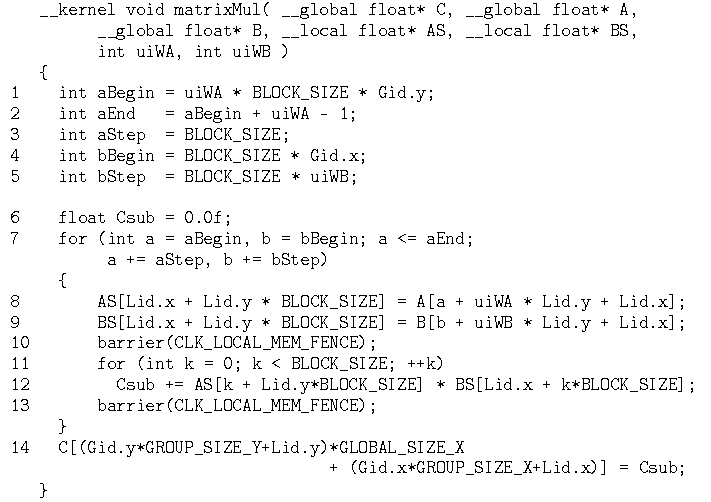
\includegraphics[width=12cm]{fig1-3.pdf}}
	\label{orgkernel}
\end{table}

下面以实例来说明本节所采用的数组访问描述式。
表\ref{orgkernel}为来自Nvidia GPU Computing SDK的矩阵乘法OpenCL Kernel程序,它面向GPU实现了$\bm{C}=\bm{A}\times \bm{B}$。
为了清晰易懂,原Kernel中的一些变量名被修改,此外,{\tt Lid} 代表工作项的局部索引值,{\tt Gid}代表工作组的组索引值。
在Kernel的外层循环中(第7$\sim$13行),一共有6处数组访问:
第8行的写$\bm{AS}$和读$\bm{A}$,
第9行的写$\bm{BS}$和读$\bm{B}$,
第12行的读$\bm{AS}$和读$\bm{BS}$。
作为示例,对于$\bm{AS}$和$\bm{A}$的3处数组访问的线性描述式如图\ref{desriptor1}所示。
其中,$f$代表线性下标函数,$Constraint$代表线性访问约束的集合,
$Iter_x$($x = a, b, k$)代表循环正规化(Loop Normalization)后的循环变量。
对于数组访问$\texttt{A[a + uiWA * Lid.y + Lid.x]}$,得到的线性下标函数是$f^{read}_{A}$,其值覆盖了Kernel执行时对数组$\bm{A}$的所有可能的访问位置。
线性约束集合$Constraints^{read}_{A}$通过约束$f^{read}_{A}$中变量的取值,限制了上述访问位置的范围。
对于数组$\bm{BS}$和$\bm{B}$ 的访问描述式与图\ref{desriptor1}非常类似,因此不再单独列出。

\begin{figure}[htb]
	\scalebox{0.8}{$\left\{ \begin{array}{l}
		f_{\bm{A}}^{read} = (uiWA \times BLOCK\_SIZE \times Gid.y + BLOCK\_SIZE \times Ite{r_a}) + uiWA \times Lid.y + Lid.x\\
		Constraint_{\bm{A}}^{read} = \{ Ite{r_a} \ge 0\;;\;\;Ite{r_a} < uiWA/BLOCK\_SIZE;\;Gid.y \ge 0;\;\\
		\;\;\;\;\;\;\;\;\;\;\;\;\;\;\;\;\;\;\;\;\;\;\;\;\ \ \ \ \ \ Gid.y < GLOBAL\_SIZE; \ 
		Lid.x \ge 0;\;Lid.x < BLOCK\_SIZE;\;Lid.y \ge 0;\\
		\;\;\;\;\;\;\;\;\;\;\;\;\;\;\;\;\;\;\;\;\;\;\;\;\ \ \ \ \ \ Lid.y < BLOCK\_SIZE\} 
		\end{array} \right.$}
	\vspace{0.1in}
	
	\scalebox{0.8}{$\left\{ \begin{array}{l}
		f_{\bm{AS}}^{write} = Lid.x + Lid.y \times BLOCK\_SIZE\\
		Constraint_{\bm{AS}}^{write} = \{ Lid.x \ge 0;\;Lid.x < BLOCK\_SIZE;\;Lid.y \ge 0;\;Lid.y < BLOCK\_SIZE\} 
		\end{array} \right.$}
	\vspace{0.1in}
	
	%\hspace{1.025in}\scalebox{0.8}{$\left\{ \begin{array}{l}
	%f_B^{read} = (BLOCK\_SIZE \times Gid.x + BLOCK\_SIZE \times uiWB \times Ite{r_b}) + uiWB \times Lid.y + Lid.x\\
	%Constraint_A^{read} = \{ Ite{r_b} \ge 0;\;\;Ite{r_b} < uiWB/BLOCK\_SIZE;\;Gid.x \ge 0;\;Gid.x < GLOBAL\_SIZE;\\
	%\;\;\;\;\;\;\;\;\;\;\;\;\;\;\;\;\;\;\;\;\;\;\;\;\ \ \ \ \ \ \ Lid.x \ge 0;\;Lid.x < BLOCK\_SIZE;\;Lid.y \ge 0;\;Lid.y < BLOCK\_SIZE\} 
	%\end{array} \right.$}
	%
	%\hspace{1.03in}\scalebox{0.8}{$\left\{ \begin{array}{l}
	%f_{BS}^{write} = Lid.x + Lid.y \times BLOCK\_SIZE\\
	%Constraint_{BS}^{write} = \{ Lid.x \ge 0;\;Lid.x < BLOCK\_SIZE;\;Lid.y \ge 0;\;Lid.y < BLOCK\_SIZE\} 
	%\end{array} \right.$}
	%\vspace{0.05in}
	
	\scalebox{0.8}{$\left\{ \begin{array}{l}
		f_{\bm{AS}}^{read} = Ite{r_k} + Lid.y \times BLOCK\_SIZE\\
		Constraint_{\bm{AS}}^{read} = \{ Ite{r_k} \ge 0;\;\;Ite{r_k} < BLOCK\_SIZE;\;Lid.y \ge 0;\;Lid.y < BLOCK\_SIZE\} 
		\end{array} \right.$}
	
	%\hspace{1.03in}\scalebox{0.8}{$\left\{ \begin{array}{l}
	%f_{BS}^{read} = Lid.x + Ite{r_k} \times BLOCK\_SIZE\\
	%Constraint_{BS}^{read} = \{ Ite{r_k} \ge 0;\;\;Ite{r_k} < BLOCK\_SIZE;\;Lid.x \ge 0;\;Lid.x < BLOCK\_SIZE\} 
	%\end{array} \right.$}
	\caption{矩阵乘法Kernel中读$\bm{A}$、写$\bm{AS}$和读$\bm{AS}$的数组访问线性描述式}
	\label{desriptor1}
\end{figure}

有了本节中提出的数组访问线性描述式的帮助,
对GPU特定OpenCL Kernel程序的代码转换将分为两步进行:
基于分析的工作项折叠和适应体系结构的后继优化。
这两步的目的都是提升Kernel程序在多核/众核CPU上的性能。

\section{基于分析的工作项折叠}
\label{kernelcoalescingsec}
工作项折叠(或者串行化)的目的是加粗线程粒度,通常会将一个工作组内的所有工作项合并为一个独立的CPU线程。
标准的折叠方法是构建线程循环嵌套。
该循环嵌套的层数和Kernel的索引空间维度一致,
各层的循环变量与工作项的局部索引对应,最内层的循环体就是原Kernel程序,如图\ref{serialize}(a)、(b)所示。

但是构建这样的线程循环并非易事,面临的最大挑战就是Kernel程序中同步语句(如\texttt{barrier()})的存在。
当前最先进的工作项折叠方法均采用循环分裂来解决同步问题。
图\ref{serialize}(c)、(d)展示了构建线程循环并使用循环分裂的例子。
图\ref{serialize}(d)中,由于\texttt{barrier()}语句的存在,线程循环在同步语句处被分裂为两个线程循环。
循环分裂所带来的额外开销主要有两部分,一是额外的循环控制语句,
二是可能导致的变量扩展(Variable Expansion)。
变量扩展指的是,当分裂出的两个循环的循环体中有共用变量时,由于执行路径的改变,需要保存第一个循环每次迭代后的共用变量值。
否则,第二个循环得到的将只有前一循环最后一次迭代得到的共用变量值。
如果工作组内的工作项数目较多,变量扩展将导致大量的额外访存开销(变量将无法放入寄存器中)。
为此,本节将基于数组访问描述式进行准确的工作项间依赖性分析,将不必要的同步语句预先消除,
从而从根本上避免循环分裂。具体细节将在\ref{dependenceanalysissec}节中介绍。

\begin{figure}[htb]
\centering
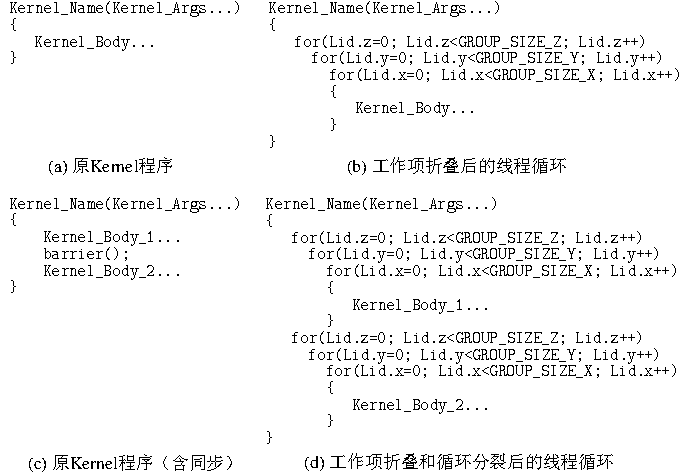
\includegraphics[width=13.25cm]{fig3.pdf}
\caption{通过构建线程循环来进行工作项折叠}
\label{serialize}
\end{figure}

工作项折叠过程中,另一极大影响性能的要素就是OpenCL局部存储的使用。
使用在局部存储中分配的数组是GPU特定Kernel程序非常常用的性能优化方法。
因为OpenCL局部存储直接对应着GPU的高速片上存储,访问局部存储数组会十分高效。
但是,CPU体系结构中并没有能够与局部存储对应的硬件支持,因此现有的OpenCL运行时只能用一段主存空间来模拟局部存储的功能。
在这种情况下,如果不加区分地使用局部存储数组,很可能由于额外的数据拷贝和附带的同步,导致性能反而下降。
目前已有的工作项折叠方法均没有对局部存储数组进行有效的处理,
而本节的一大创新就是在折叠过程中去除冗余的局部存储数组,从而提升Kernel程序性能。
对局部存储数组是否冗余的相关分析,以及对应的去除过程,都是基于数组访问描述式的,
具体将在\ref{localmemeliminatesec}节中进行介绍。

\subsection{去除冗余的局部存储数组}
\label{localmemeliminatesec}
局部存储数组在GPU特定的OpenCL Kernel程序中的作用可以分为以下4种类型:
\begin{compactitem}
\item[1)]{\textbf{数据缓存}:为了提升Kernel程序的时间和空间局部性,将经常访问或者将被重复访问的数据缓存在局部存储中,从而使延迟较长的全局存储访问变为更快速的局部存储访问。}
\item[2)]{\textbf{数据重组}:通过合并访存的方式从全局存储中读出数据,然后以另一种形式存入局部存储中,以避免后续对局部存储的访问发生组冲突(Bank Conflict)。一个典型的例子就是矩阵转置相乘($\bm{C} = \bm{A}\times \bm{A}^{\rm T}$)Kernel\upcite{oclbestpractice}中,$\bm{A}$按行从全局存储中读出,之后按列存入局部存储数组。}
\item[3)]{\textbf{数据交换}:将工作项执行的中间结果存入局部存储中,然后由其它工作项读出。这种作用类型不仅能够在工作项间交换数据,还能避免多个工作项进行重复的计算。}
\item[4)]{\textbf{防止寄存器溢出}:如果Kernel内申请的私有变量过多,导致执行所有工作项所需的寄存器不足,那么这些私有变量就会溢出到低速的片外存储(显存)内,导致性能大幅下降。这种作用类型将局部存储看作是私有存储的扩展,用于存储更多的工作项私有数据。 }
\end{compactitem}

在CPU体系结构下,第3)种作用类型的OpenCL局部存储数组也是必需的,
因此在工作项折叠过程中不可去除。
具有第4)种作用的局部存储数组也不可去除,因为该局部存储数组是用于存放中间结果的,一旦去除将无处存放溢出的数据。
对于第2)种作用类型的局部存储数组,尽管CPU只是用一段主存空间进行模拟,并且会导致一次额外的数据拷贝,本节也仍然将其保留。
原因在于其中的数据进行过重组,后续的访存将变得高效,从而很可能提升最终性能。
至于第1)种作用类型,局部存储数组就完全多余了。
因为CPU体系结构中的多级Cache具有完全相同的功能,所以使用局部存储数组是毫无意义的,还会导致额外的数据拷贝。
要准确去除第1)种作用类型的数组,需要首先通过分析判别局部存储数组的作用类型,然后将对原数组的访问转换为对全局存储数组的访问。

如果一个局部存储数组不具备第3)和第4)种作用,但是具备第1)或者第2)种(又或两种皆有之),
那么Kernel程序对它的一系列访问必然满足下列过程\upcite{oclprogrammingguide}:
\begin{compactitem}
\item[$\rightarrow$]{从全局存储数组中读出数据,再存入该局部存储数组中。} 
\item[$\rightarrow$]{可能在工作组内进行一次同步,以确保之后每个工作项都可以安全地读取到其它工作项写入的数据。} 
\item[$\rightarrow$]{从该局部存储数组中读出数据,并使用数据进行计算。} 
\item[$\rightarrow$]{如果访存过程是循环的,则还需要一次同步,以避免有的工作项还未利用该局部存储数组中的数据进行计算。}
\end{compactitem}
例如表\ref{orgkernel}中,$\bm{AS}$和$\bm{BS}$这两个局部存储数组就是仅用于缓存数据的。
对这两个数组的访问完全符合上述过程。
如表\ref{orgkernel}的第8、9行所示,数组$\bm{AS}$和$\bm{BS}$中的数据直接来自于全局存储数组$\bm{A}$和$\bm{B}$。
而第10、13行即是所需的两次同步。

只有当同时满足下列两个条件时,局部存储数组的读访问才能被转换为直接的全局存储数组读访问:
\begin{compactitem}
\item[(1)]{存在一个与该局部存储数组读访问相对应的局部存储数组写访问:如果将写访问的描述式中的某些变量替换为读访问中的变量,二者的数组访问描述式(包括下标函数和访问约束)可变得完全相同。}
\item[(2)]{(1)中的局部存储数组写访问的数据是来自于全局存储数组的。该条件可以通过检查``定义—使用链(Define-Use Chain)\upcite{compilerbook2}''来验证,且通常情况下,局部存储数组写访问和对应的全局存储读访问是相邻的。}
\end{compactitem}
如果一个局部存储数组具有作用类型3)或者4),那么对它的读访问将无法满足上述两个条件,因为数组中的元素均来自于中间计算结果,而不是来自全局存储。

将局部存储数组的读访问转换为全局存储数组读访问的过程,
就是找出所有满足上述两个条件的局部存储数组读操作,然后将它们用条件(2)中的全局存储数组读操作替换。
随后,与条件(1)中的局部存储数组写访问相关的语句将变为``死代码(Dead Code)'',被编译器自动地去除。
一个典型的例子就是图\ref{desriptor1}中的那对局部存储数组读写:
%\begin{small}
\begin{equation}
\small
\left\{ \begin{array}{l}
f_{\bm{AS}}^{write}=Lid.x + Lid.y \times BLOCK\_SIZE\\
Constraint_{\bm{AS}}^{write}=\\ \{ Lid.x \ge 0;\;Lid.x < BLOCK\_SIZE;\ Lid.y \ge 0;
\\ \;Lid.y < BLOCK\_SIZE\} 
\end{array} \right.,
\label{eq4.1}
\end{equation}
\begin{equation}
\small
\left\{ \begin{array}{l}
f_{\bm{AS}}^{read} = Ite{r_k} + Lid.y \times BLOCK\_SIZE\\
Constraint_{\bm{AS}}^{read} = \\
\{ Ite{r_k} \ge 0;\;\;Ite{r_k} < BLOCK\_SIZE;\ Lid.y \ge 0;\\ \;Lid.y < BLOCK\_SIZE\} 
\end{array} \right..
\label{eq4.2}
\end{equation}
%\end{small}
如果将公式(\ref{eq4.1})中的$Lid.x$ 用公式(\ref{eq4.2})中的$Iter_k$ 替换,那么上面两个数组访问描述式将变得一样,即满足了条件(1)。
此外,根据表\ref{orgkernel}第8行,公式(\ref{eq4.1})的数据来源是全局存储数组$\bm{A}$ :
\begin{equation}
\small
\begin{array}{l}
f_{\bm{A}}^{read} = (uiWA \times BLOCK\_SIZE \times Gid.y + \\ BLOCK\_SIZE \times Ite{r_a})
 + uiWA \times Lid.y + Lid.x,
\end{array}
\label{eq4.3}
\end{equation}
因此条件(2)也满足了。
综上,将公式(\ref{eq4.2})对应的局部存储数组读访问转换为直接的全局存储数组读访问是可行的。
通过将公式(\ref{eq4.3})中的$Lid.x$替换为$Iter_k$,然后用变量替换后对应的读操作代替公式(\ref{eq4.2})对应的读操作,即可完成转换:
\begin{equation}
\begin{array}{l}
\small
f_{\bm{AS}}^{read} = Ite{r_k} + Lid.y \times BLOCK\_SIZE\\
 \Rightarrow \\
f_{\bm{A}}^{read} = (uiWA \times BLOCK\_SIZE \times Gid.y +\\ BLOCK\_SIZE \times Ite{r_a})
 + uiWA \times Lid.y + Ite{r_k}
\end{array}.
\end{equation}

上述的转换条件和方法只考虑了可行性,即可用于所有没有数据交换功能和防止寄存器溢出功能的局部存储数组。
但是,对于具有数据重组功能的局部存储数组,上述方法虽然可行但不会带来性能提升。
因此这里再附加一个启发式的条件,以确保局部存储数组不具有数据重组的作用:
\begin{compactitem}
\item[(3)]{考察条件(1)中的局部存储数组写访问,以及(2)中的全局存储数组读访问,它们的下标函数中变量$Lid.x$必须具有相同的系数(或者都不含变量$Lid.x$,即系数为$0$)。}
\end{compactitem}
例如,在公式(\ref{eq4.1})和(\ref{eq4.3})中,下标函数$f^{write}_{\bm{AS}}$和$f^{read}_{\bm{A}}$的$Lid.x$ 变量系数均为$1$,
并且公式(\ref{eq4.1})和公式(\ref{eq4.2})覆盖了Kernel对局部存储数组 $\bm{AS}$的所有访问。
因此基于条件(3),可以确定局部存储数组$\bm{AS}$不具有数据重组的作用,
去除它将在CPU体系结构下带来性能提升。

通过去除所有仅具有数据缓存作用的局部存储数组,并且将对于这些数组的访问转换为对全局存储数组的直接访问,
工作项折叠后的Kernel性能将获得明显提升。
表\ref{localmemremoved}(代码的行号与表\ref{orgkernel}一致)展示了去除冗余的局部存储数组后的矩阵乘法代码。
其中,局部存储数组$\bm{AS}$和$\bm{BS}$由于仅作为数据缓存使用,都被去除掉了。

\begin{table}[htb]
\centering
\caption{去除冗余的局部存储数组后的矩阵乘法Kernel代码片段}
\fbox{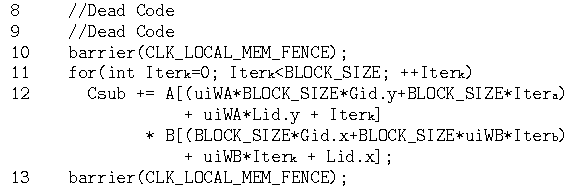
\includegraphics[width=10cm]{fig4.pdf}}
\label{localmemremoved}
\end{table}

\subsection{依赖性分析和同步语句消除}
\label{dependenceanalysissec}
如果一个工作组中的不同工作项会访问相同的存储位置,那么同步通常是必要的,否则Kernel程序的执行结果将是不确定的。
在Kernel程序中,作为同步点的\texttt{barrier}语句经常会离局部存储数组的访问非常近,这是因为局部存储是由工作组内的所有工作项所共享的存储空间。
但是,\texttt{barrier}语句的存在并不代表工作项间确实存在依赖性(写后读相关、读后写相关、或写后写相关),而由于依赖所产生的同步才是真正不可消除的。
例如,\ref{localmemeliminatesec}节所述的4种局部存储数组作用类型中,只有数据交换才会导致真正的数据依赖,
即一个工作项在获取到另一工作项的中间结果前,无法继续执行。
具有其它3种作用类型的局部存储数组也可能引入同步语句,但是工作项间并没有真正的依赖性。
如果各个工作项直接从全局存储中获取所需的数据,同步语句则不再必要。
也即是说,如果\texttt{barrier}语句是由仅具有数据缓存或数据重组功能的局部存储数组引入的,那么它是可以随着局部存储数组一起去除掉的。

在CPU体系结构下,同步语句的作用可能存在两面性。
工作项折叠时,如果在同步语句位置进行循环分裂,则一定会导致额外的开销,如循环控制和变量扩展。
但是循环分裂的同时也改变了工作组的执行流程,从而也可能带来更好的时间和空间局部性。
对于这个两面性问题,本节的解决方案是:
在工作项折叠过程中忽略同步语句可能带来的好处,尽可能地去除同步语句。
然后在线程循环的后继优化中针对具体的体系结构细节,重新开发数据局部性,具体将在\ref{localityreexploresec}节中介绍。

在去除了冗余的局部存储数组之后,就可以开始进行同步语句的消除。
但是,单纯地删除所有的\texttt{barrier}语句是不安全的,因为同步语句可能还服务于其它未被去除的局部存储数组,也可能是由于全局存储数组而导致的同步。
为了检查一个同步语句是否可以被安全地删除,需要进行依赖性分析。
这里的依赖性分析和经典的依赖性分析有很大的不同,因为它是在不同的工作项间进行的。
而在工作项内代码是串行执行的,因此无需考虑工作项内的依赖性,该依赖性也与同步无关。
本节依赖性分析的核心思想是:如果两个工作项访问了同一局部存储数组或全局存储数组(其中至少有一个访问是写访问),
并且访问的数组区域有重叠,那么这两个工作项间就存在依赖性。

依赖性分析是针对每一条\texttt{barrier}语句逐次进行的。
首先将同步语句也看作是基本块(Basic Block)边界,将Kernel代码划分为多个基本块。
虽然引入了同步,但是这里基本块的概念和经典编译理论中的概念是一致的,
即基本块是一个包含了尽量多的语句的代码段,其中任意一条语句的执行,意味着块内的其它语句也一定会执行。
然后需要考察每一对满足下列条件的数组访问:
两个数组访问分别来自位于同步语句前、后的基本块;两个数组访问针对同一个局部存储数组或全局存储数组;
其中一个数组访问是写访问。
如图\ref{dependence}的上半部分所示,虚线矩形框代表的是不同控制语句导致的基本块划分,箭头指向的是需要考察其中数组访问的两个基本块。
图\ref{dependence}的下半部分强调了对数组访问的考察是针对不同工作项的。
考察一对数组访问时,需要将二者对应的数组访问描述式进行联立,构成一个丢番图不等式系统(Diophantine Inequation System)。
如果该不等式系统有解,且解中不要求所有的工作项局部索引值相等,那么真正的依赖存在,对应的\texttt{barrier}语句不可删除。

\begin{figure}
	\centering
	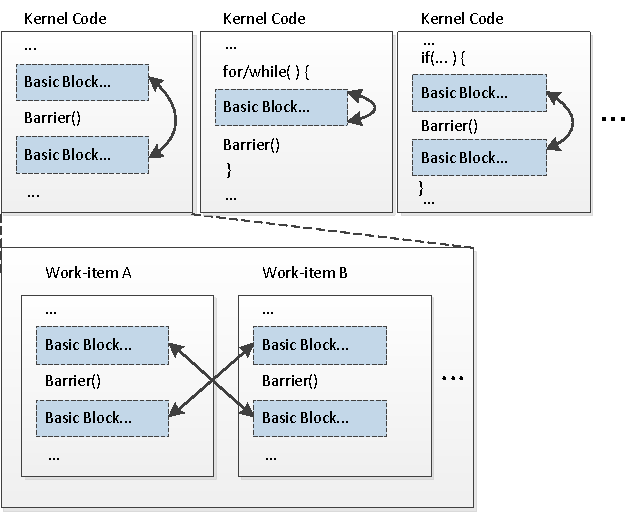
\includegraphics[width=10.5cm]{fig5.pdf}
	\caption{依赖性分析示意图}
	\label{dependence}
\end{figure}

公式(\ref{eq4.5})展示了上述不等式系统的构建过程:
\begin{equation}
\small
\begin{array}{l}
\left\{ \begin{array}{l}
{f_1} = \overrightarrow {\bm{Co{e_1}}}  \cdot {\overrightarrow {\bm{Var_1}}}^{\rm T} + Const\\
Constrain{t_1}
\end{array} \right. \hspace{0.2in}{\overrightarrow {\bm{Var_1}}} = (...,Lid.z,Lid.y,Lid.x)\\
\\ 
\left\{ \begin{array}{l}
{f_2} = \overrightarrow {\bm{Co{e_2}}}  \cdot {\overrightarrow {\bm{Var_2}}}^{\rm T} + Const\\
Constrain{t_2}
\end{array} \right. \hspace{0.2in}{\overrightarrow {\bm{Var_2}}} = (...,Lid.z',Lid.y',Lid.x')\\
\\ 
\Rightarrow \left\{ \begin{array}{l}
{f_1} = {f_2}\\
Constrain{t_1}\\
Constrain{t_2}
\end{array} \right.
\end{array}.
\label{eq4.5}
\end{equation}
其中$\overrightarrow{\bm{Coe}}$代表变量系数组成的向量,
$\overrightarrow{\bm{Var}}$代表变量组成的向量,$Const$代表一个常数。
需要注意的是,由于依赖性分析针对的是两个不同的工作项,$\overrightarrow{\bm{Var_1}}$和$\overrightarrow{\bm{Var_2}}$中的工作项局部索引值不再被看作是相同的变量,
因此这里进行了换名。
如果箭头右侧的不等式系统有解,且解中不要求$\{Lid.x=Lid.x'; Lid.y=Lid.y'; Lid.z=Lid.z'\}$,那么对应的\texttt{barrier}语句就必须保留。

通过上述的依赖性分析,所有可消除的同步语句都将被删除,继而可使用经典的工作项折叠方法,生成线程循环。
对于不可消除的同步语句,仍然采用循环分裂解决。
表\ref{debarriered}展示了工作项折叠后的矩阵乘法Kernel,
原Kernel中的两个\texttt{barrier}语句均被消除了。
从表\ref{debarriered}可以看出,同步将不带来任何直接开销。

\begin{table}[htb]
	\centering
	\caption{工作项折叠后的矩阵乘法Kernel代码片段}
	\fbox{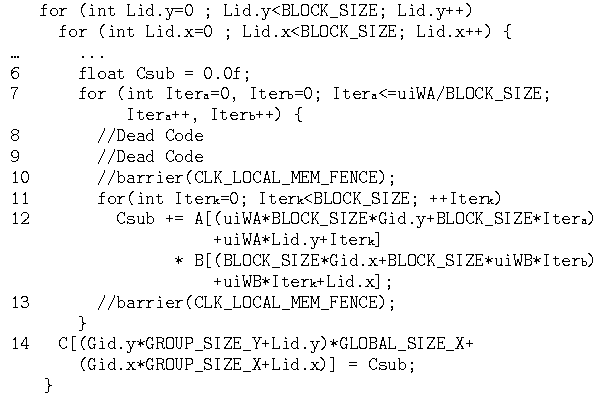
\includegraphics[width=10cm]{fig6.pdf}}	
	\label{debarriered}
\end{table}

消除同步语句之后,虽然其直接开销也被消除了,但是整个工作组的代码执行顺序也发生了改变。
图\ref{access}(a)显示了原GPU特定Kernel在执行过程中,一个工作组对于全局数组$\bm{A}$和$\bm{B}$的访问顺序。
其中粗箭头代表对数组元素的依次访问,黑色虚线箭头代表控制流。
由于采用分块矩阵乘法,$\bm{A}$的每一行分段会被连续访问16次,
$\bm{B}$的每一分块的各个行将以合并访存的方式被循环访问16次。
图\ref{access}(b)显示了工作项折叠后,线程循环的访问顺序。
矩阵乘法不再是分块的,对数组$\bm{A}$的访问将遍历整个行,对数组$\bm{B}$的访问将遍历整个列。
因此,Cache失效将不可避免,而且SIMD并行性无法得到开发。
这样的工作项折叠后代码虽然不够高效,但是十分``整齐'',有利于后继优化。
本章后继优化的目标不是还原图\ref{access}(a)所示的GPU特定的局部性,
而是根据目标CPU的体系结构细节,重新开发数据局部性和并行性。

%In Fig.~\ref{access}(c), each scalar element of $\bm{A}$ is expanded into a vector, and each set of eight adjacent accesses to $\bm{B}$ is vectorized to produce a new vector. Then computational operations are fully vectorized. In addition, the iterative array accesses are restricted in small blocks, so that the CPU cache can play a very good role.

\begin{figure}[htb]
\centering
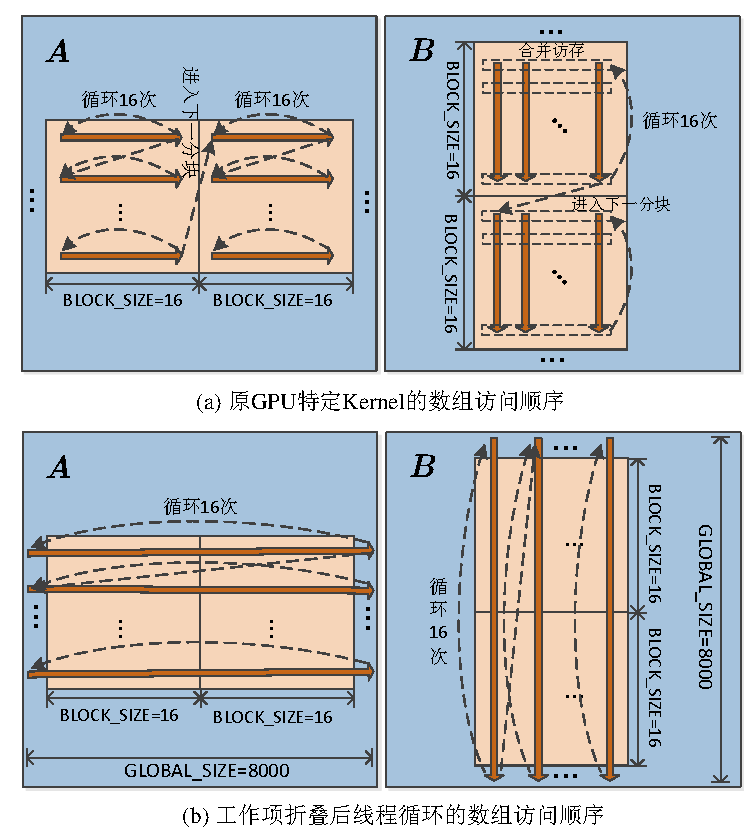
\includegraphics[width=12cm]{fig7.pdf}
\caption{矩阵乘法$\bm{C}=\bm{A}\times \bm{B}$中对于数组$\bm{A}$和$\bm{B}$的不同访问顺序}
\label{access}
\end{figure}


\section{适应体系结构的后继优化}
\label{postoptimizationsec}
完成工作项的折叠后,线程粒度大大变粗,工作组能够以线程循环的形式作为一个CPU线程进行执行。
但是此时仍然有两个CPU特定的性能要素没有得到利用。
一个是工作项间的并行性没有得到开发,导致CPU中的SIMD单元利用率低下。
另一个是线程循环的循环体过长,导致数据局部性不佳。
为此,本节将对折叠后的线程循环进行两步优化:向量化和局部性重开发。
这两步优化的目的在于,借鉴原GPU特定Kernel对于性能的考虑,针对CPU特定的体系结构细节提升代码性能。

\subsection{向量化}
对于工作项折叠后的线程循环,{\em icc}等高性能编译器能够进行自动向量化,以利用当前多核/众核CPU中广泛存在的SIMD单元。
但是,编译器通常只针对循环嵌套的最内层循环进行向量化\upcite{intelvectorguide},
而最内层循环可能无法向量化,或者不是进行向量化的最佳位置。
因此本节将不依赖编译器的自动向量化功能,而是显式地进行循环级的向量化优化。
这一过程不仅需要提取原GPU特定Kernel中的并行信息,同时还会考虑CPU的体系结构细节。

对于GPU来说,访问全局存储数组的最佳模式是顺序、逐个、对齐的访问\upcite{oclbestpractice}。
例如,第$k$个工作项访问对齐的全局存储段的第$k$个字。
这样的访存模式必然是合并访存,可以最大化地利用GPU的显存带宽。
GPU特定Kernel程序对于局部存储数组的访问通常也是顺序、逐个的(无需对齐),
目的是避免访存时发生组冲突。
此外,GPU还有一种高效的局部存储访问模式,即令同一Warp$/$半Warp内的工作项访问同一局部存储位置。

由于CPU体系结构下,OpenCL的全局存储和局部存储均对应于主存,
因此最适于进行向量化的循环层次就是以$Lid.x$为循环变量的循环。
原因在于,该层循环的相邻迭代对应于相邻的工作项。
而相邻工作项顺序、逐个的访存模式正好可以转换为向量加载指令(Vector-Load)和向量存储指令(Vector-Store);
相邻工作项访问同一存储位置的访存模式也可以转化为置向量指令(Vector-Set)或向量广播指令(Broadcast)。
除了访存操作以外,各种数学操作都可以通过经典的循环向量化方法无障碍地进行向量化,因为$Lid.x$循环在工作项折叠之后,
没有任何循环间依赖。

对于工作项折叠后的代码的向量化步骤如下:
\begin{compactitem}
\item[1)]{如果原GPU特定Kernel程序中包含循环,则进行循环分布(Loop Distribution),使得非线程循环(即循环变量不是工作项索引的循环)成为循环嵌套的最内层循环。该步骤可能需要变量扩展,并会导致更多的循环控制语句。但是相比向量化后的巨大性能提升,这些额外开销是可忽略的。}
\item[2)]{对于每一个循环嵌套,进行循环交换(Loop Interchange),使得$Lid.x$循环成为循环嵌套的最内层循环。这一步骤一定是可进行的,因为线程循环的循环层间没有任何依赖。}
\item[3)]{根据目标CPU体系结构的SIMD单元宽度,对$Lid.x$循环进行循环分段(Loop Blocking),使得得到的循环嵌套的外层循环变量(记为$vLid.x$ )以(SIMD单元宽度$/$数组元素宽度)为步长。之后即可按经典方法对最内层循环进行向量化。假设用于计算的是单精度浮点数(32位),对于Sandy Bridge架构的CPU,由于SIMD宽度为256位,循环步长设为8。而对于Knights Corner架构的MIC协处理器,由于SIMD宽度为512位,循环步长设为16。此外Knights Corner架构还包括了向量乘加单元(FMA),因此其编译器可以自动地将乘法和加法融合。}
\end{compactitem}

工作项折叠后的矩阵乘法Kernel代码,再经过向量化,变为如表\ref{vectorized}所示。
表中假设CPU的SIMD宽度为256位,所示的$vLid.x$是经过了循环正规化的。
前缀``vec''代表向量数据类型或者向量操作。
可以看出,$Lid.x$循环被分段后得到的3个循环嵌套中,最内层的循环都已经因为完全向量化而消失了。

\begin{table}[htb]
\centering
\caption{向量化后的矩阵乘法Kernel代码片段}
\fbox{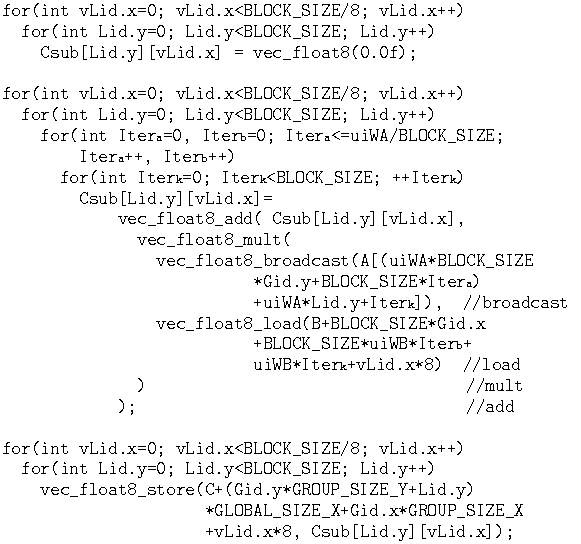
\includegraphics[width=10cm]{fig8.pdf}}
\label{vectorized}
\end{table}

\subsection{局部性重开发}
\label{localityreexploresec}
经过工作项折叠和向量化,转换得到的Kernel程序的并行性已经非常适合CPU体系结构。
但是,数据局部性仍然没有得到改善。
大部分的GPU特定Kernel程序在实现时都考虑了数据局部性,例如将长循环分段等。
但是有的Kernel程序并没有进行相关优化。例如\cite{oclprogrammingguide}中给出的``基本矩阵乘法Kernel'',
它和上文中讨论的矩阵乘法Kernel具有相同的功能,但是没有进行任何局部性优化,因此被Nvidia作为一个基准程序来展示局部存储的作用。
本节的局部性重开发方法会利用到原GPU特定Kernel对于局部性的优化,但同时也会尽量适应目标CPU体系结构对数据局部性的需求,
因此即使是数据局部性很差的GPU特定Kernel,仍然可以通过本节的方法在CPU上获得极大性能提升。
本节使用(并微调)了经典的循环级优化方法,包括循环交换、循环分段和提升寄存器重用率。
具体的数据局部性重开发方法分为以下3个步骤。

{\bf 1)\ 将非线程循环分段。} 主要思想是:如果一个循环的循环变量出现在了一个多维数组的最低维(该维度的相邻元素在内存中连续)索引中,且不出现在其它维度的索引中,那么对该循环进行分段通常是有好处的\upcite{compilerbook}。
对于所有的非线程循环,如果同时满足下面两个条件,则对其进行分段:
\begin{compactitem}
\item[a)]{循环体中某个数组访问对应的线性描述式包含了非线程循环的循环变量,且该循环变量的系数足够小;(这里以2作为保守的阈值,因为太大的系数会导致访存模式的步长较大,从而限制循环分段的有效性。)}
\item[b)]{对于a)中的数组访问,将一次循环迭代的元素访问范围转换为字节数,得到访存覆盖范围足够大。(这里使用一个经验阈值,即L1 Cache大小的$1/8$,因为如果每次迭代的访存范围很窄,则无需进行循环分段。对于Sandy Bridge和Knights Corner架构,该阈值均为4KB。)}
\end{compactitem}
如果需要进行循环分段,非线程循环将被转换为两个嵌套的循环,并且内层循环的迭代次数(Trip Count)将被设置为工作组最低维的工作项数目,即$Lid.x$的取值范围大小。
经典的循环分段包括两个步骤,分段开采和循环交换。但是这里的循环分段只进行分段开采,而不考虑循环交换。
循环交换将在下一步骤中,针对所有层次的循环(包括线程循环)同时进行。
如表\ref{vectorized}的中间部分所示,${Iter_k}$循环和${Iter_a/Iter_b}$循环实际上已经是非线程循环被分段后得到的内、外层循环了,
因此没有非线程循环满足上述分段条件。
但是,``基本矩阵乘法Kernel''中的$k$循环会被检测出来并进行分段处理。

{\bf 2)\ 循环交换。} 这里将沿用Allen等人提出的启发式循环交换算法\upcite{compilerbook}。
对于嵌套的多个循环$\{ {L_1}, {L_2},\ldots ,{L_n} \}$,首先建立一个启发式函数,用于估计循环嵌套中的数组访问(包括向量加载和存储)可能导致的Cache失效次数。
然后对于每一层循环${L_i}$,假设其处于最内层,用启发式函数估计出循环嵌套的Cache失效次数(称作该循环的最内层存储开销),记为$C_M({L_i})$。
最后,各层循环按照$C_M$值的降序,从内到外进行重新排列。

但是,上述循环交换算法在计算$C_M$值时基于一个重要假设,即当前循环的迭代次数是无限大的。
而线程循环和分段后的内层非线程循环的迭代次数通常较少,因此上述算法还需要修改:
当计算一个循环的最内层存储开销(即$C_M$值)时,如果它的迭代次数少于工作组最低维的工作项数目,则不再把它的失效次数乘以它外层循环的迭代次数。
上述算法有的时候还会产生多个循环交换方案,例如表\ref{vectorized}中间部分的嵌套循环中,
${Iter_a/Iter_b}$循环应当被置于最外层,${Iter_k}$循环应当被置于最内层,而${vLid.x}$循环和${Lid.y}$循环的位置是可以互相交换的。

{\bf 3)\ 选择利于向量寄存器重用的循环交换。} 单个CPU核里的向量寄存器是非常稀有的计算资源。Sandy Bridge架构中有16个,
Knights Corner架构中有32个。因此向量寄存器的重用率将对Kernel性能产生很大影响。
提升寄存器的重用率实际上就是提升Kernel的数据时间局部性,故这里仍然利用上一步中计算$C_M$值的启发式函数,
并针对时间局部性进行修改:
每一个向量操作都被看作是``访存操作'',Cache大小设置为向量寄存器的数量,Cache行的长度设置为$1$。
这样一来,修改后的启发式函数估计出的``Cache失效次数''实际上是向量寄存器的溢出次数。
将该启发式函数应用于上一步得到的所有循环交换方案,$C_M$值最小的方案就是向量寄存器重用率最高的循环交换。
再次观察表\ref{vectorized}中间部分的嵌套循环,如果一个CPU核包含16个256位的向量寄存器,
那么将${vLid.x}$循环置于${Lid.y}$循环之外将获得更佳的时间局部性。

经过局部性重开发后的矩阵乘法Kernel代码片段如表\ref{cpuoutput}所示(仅显示了Kernel中间的循环嵌套),
它同时也是将GPU特定Kernel面向Sandy Bridge架构的CPU转换所得到的最终结果。
对于数组$\bm{A}$和$\bm{B}$的访问顺序也变为图\ref{access2}所示。
可以看出,原GPU特定Kernel中的合并访存转换为了向量操作,数据局部性也得到了大幅提升。

\begin{table}[htb]
	\centering
	\caption{面向Sandy Bridge架构转换后的最终矩阵乘法Kernel代码片段}
	\fbox{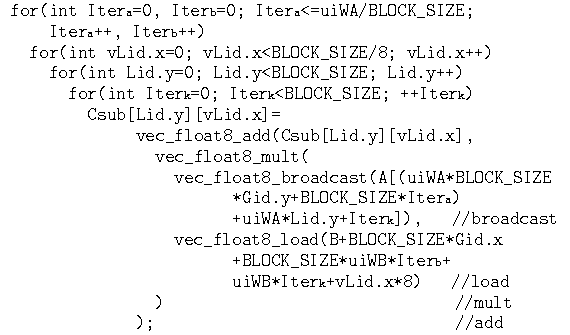
\includegraphics[width=10.5cm]{fig9.pdf}}
	\label{cpuoutput}
\end{table}

\begin{figure}[htb]
\centering
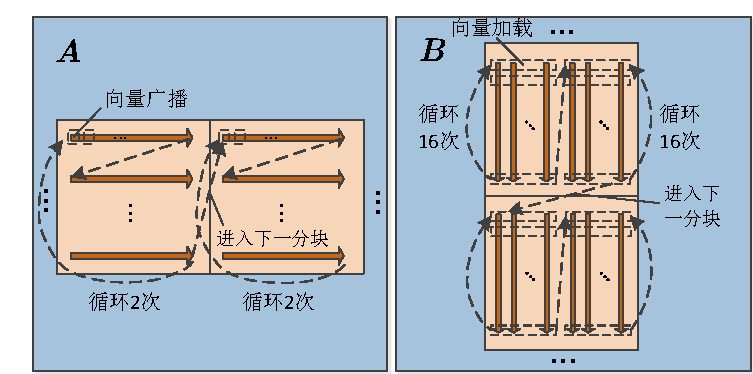
\includegraphics[width=12cm]{fig72.pdf}
\caption{转换后的矩阵乘法Kernel对于数组$\bm{A}$和$\bm{B}$的访问顺序}
\label{access2}
\end{figure}

表\ref{micouput}显示了将GPU特定Kernel面向Knights Corner架构的MIC转换所得到的最终结果。
其中${vLid.x}$循环和${Lid.y}$循环的位置可以互换,不影响性能。
表\ref{micouput}和表\ref{cpuoutput}有区别的原因在于不同的SIMD宽度、是否有FMA单元、以及不同的向量寄存器数量。


\begin{table}[htb]
\centering
\caption{面向Knights Corner架构转换后的最终矩阵乘法Kernel代码片段}
\fbox{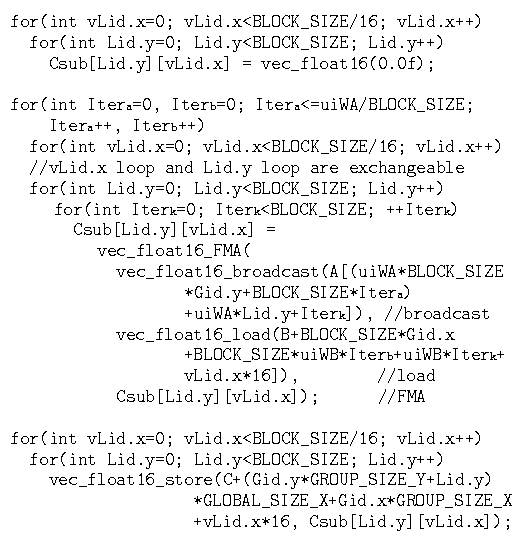
\includegraphics[width=10cm]{fig10.pdf}}
\label{micouput}
\end{table}


\section{运行时调度}
\label{runtimesec}
上述的整个代码转换过程,包括提取数组访问描述式,消除冗余的局部存储数组和同步语句,构建线程循环,
以及后继优化,被实现为一个源到源的代码转换工具链。
该工具链基于Clang\upcite{clang}编译器前端,以及LLVM\upcite{llvm}中间代码转换库。
通过工具链的转换,再利用LLVM的CBE后端,GPU特定的OpenCL Kernel程序被转换为一个可链接的函数,
其输入参数为原Kernel的全部参数和工作组的组索引值。
每一次调用该函数,等价于执行了一个对应的工作组,也就是说,
进行运行时调度的粒度为单个工作组。

转换得到的Kernel代码不能直接被标准的OpenCL运行时调度运行。
因此需要一个配套的运行时调度器来调用转换后的函数。
该调度器的功能应类似于标准OpenCL运行时对工作组的调度。
本节实现调度器的主要思想是,将工作组尽可能连续地和均匀地分布到各个CPU核上执行,
即是说各个CPU核分到的工作组数量差别不超过$1$。
通过调度器,工作组间的并行性被转换为了线程级的并行性。

调度器执行Kernel的过程如下:
\begin{compactitem}
\item[1)]{主线程将所有工作组分成多个等量的集合,各个集合被连续地指派到目标多核/众核CPU的各个逻辑核上。
(由于超线程(Hyper Thread)技术,Sandy Bridge架构下一个物理核等价于两个逻辑核,而Knights Corner架构下一个物理核等于4个逻辑核,但这里忽略其第一个物理核,以用于执行主线程。)}
\item[2)]{主线程为每一个逻辑核创建一个POSIX线程,称作工作线程。
并通过设置线程的亲和属性(Affinity)来指定工作线程在对应逻辑核上运行。}
\item[3)]{各个工作线程根据被指派的工作组,不断地以工作组组索引值为参数调用转换后的函数。}
\item[4)]{主线程等待工作线程的汇聚(Join)。}
\end{compactitem}

利用工具链转换GPU特定Kernel的过程,以及转换后的代码通过调度器运行的过程都展示在了图\ref{sysdiagram}中。

\begin{figure}[htb]
	\centering
	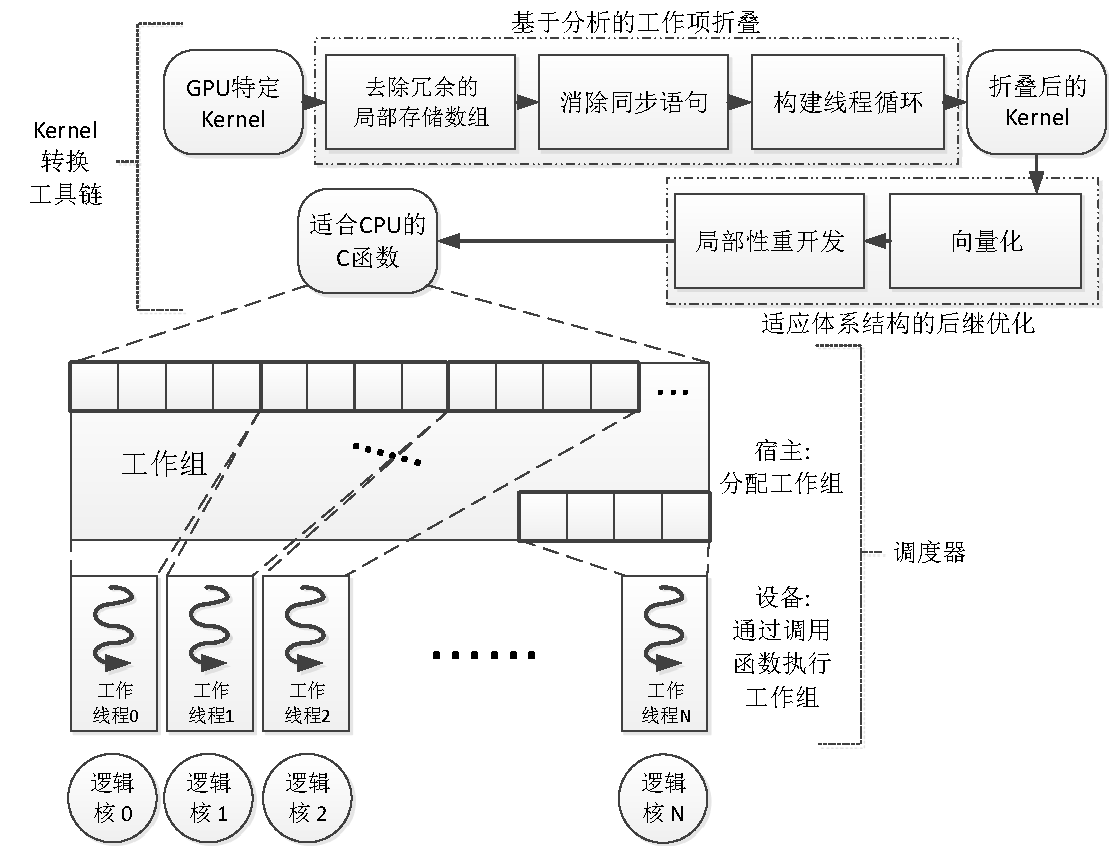
\includegraphics[width=13cm]{fig11.pdf}
	\caption{GPU特定Kernel的转换和调度执行}
	\label{sysdiagram}
\end{figure}

为了能够运行包括宿主程序和Kernel程序的完整OpenCL程序,本章的代码转换工具链和运行时调度器被集成到一个开源的OpenCL实现\pozhehao FreeOCL\upcite{freeocl}中。
原FreeOCL中的代码生成模块和Kernel调度模块被本章的代码转换工具链和调度器分别替换。
其它用于实现OpenCL宿主程序API的模块保持不变。
对于CPU和MIC,均使用Intel C++ Compiler v13.0.0编译转换后的Kernel代码。
在面向Sandy Bridge架构的CPU进行编译时,主要的编译选项为\texttt{-O3 -xHost}。
而对于Knights Corner架构的MIC,将在编译前需要为转换后的Kernel代码加上``offload''指导语句,使得整个Kernel程序可以在MIC上执行。
值得注意的是,由于本节在MIC上执行Kernel时使用的是卸载(Offload)模式,MIC的最后一个物理核将被保留,不可用于计算。
至此,包含GPU特定Kernel的OpenCL程序,将能够借助本章的新OpenCL运行时,在多核/众核CPU上高效地运行。

\section{性能评测}
\label{kernelexperimentsec}
本节将在两个硬件平台上进行实验和性能评测:
(1) 两个Intel Xeon E5-2650 8核CPU,共有16个物理核,作为经典的多核CPU平台;
(2) 一个Intel Xeon Phi 5110p MIC协处理器,共有60个物理核,作为新兴的众核CPU平台。
Xeon E5 CPU同时也作为宿主处理器,其上的操作系统为Red Hat Enterprise Linux 6.2,内核版本2.6.32-220。
本章提出的加入了Kernel转换工具链和运行时调度器的新OpenCL运行时(记作OurOCL),
将与Intel官方提供的OpenCL运行时(记作IntelOCL)进行对比。
Intel的官方OpenCL运行时来自Intel SDK for OpenCL Applications 2013\upcite{intelsdk}。

一共6个GPU特定的OpenCL Kernel程序组成了本节的测试集。
如表\ref{benchmarks}所示,前5个Kernel程序均针对GPU体系结构进行了高性能优化,
其中Stencil2D来自SHOC\upcite{shoc},其它4个来自Nvidia GPU Computing SDK。
第6个Kernel程序NaiveMatrixMul来自\cite{oclprogrammingguide},即\ref{localityreexploresec}节中介绍过的``基本矩阵乘法Kernel''。
它的数据局部性没有得到任何优化,将作为本节评测的基准。

\begin{table}[htb]
	\caption{用于性能评测的6个Kernel程序}
	\centering
	\scalebox{0.9} {
	\begin{tabular}{ p{2.7cm} p{3.7cm} p{2cm} p{6cm} }
		\toprule[1pt]
		Kernel名 & 数据规模 & 工作组大小      & 功能介绍\\
		\midrule[0.5pt]
		oclMatrixMul & $8000\times8000$ & $16\times16$ & 分块矩阵乘法\\
		%\hline
		\multirow{2}{*}{oclFDTD3d} & $320\times320\times320$,  & \multirow{2}{*}{$32\times32$} & \multirow{2}{*}{有限差分时域演化,三维模板计算}\\
		& Radius=16, Timestep=5	 &				&  \\
		%\hline
		\multirow{2}{*}{Stencil2D} & $4096\times4096$,  & \multirow{2}{*}{$16\times16$} & \multirow{2}{*}{标准的二维9点模板计算}\\
		& $1000$次迭代  &			  &		\\
		%\hline
		oclDCT8x8 & $10240\times10240$ & $32\times2$ &$8\times8$的离散余弦变换(DCT)\\
		%\hline
		oclNbody & $327680$ & $256$ & 327680个个体的引力模拟\\
		%\hline
		$*$NaiveMatrixMul & $8000\times8000$ & $16\times16$ & 未使用分块和局部存储的矩阵乘法\\
		\bottomrule[1pt]
	\end{tabular}
	}
	\label{benchmarks}
\end{table}

在Intel的产品平台上,IntelOCL通常是最为高效的OpenCL运行时。
一个Kernel依靠IntelOCL获得的性能通常也是最优的,即代表了``官方提供''的性能移植性。
因此通过对比同一Kernel在OurOCL和IntelOCL下的性能,即可评价两个运行时所提供的性能移植性。
上述的GPU特定Kernel程序在OurOCL下运行时,会先经过Kernel转换工具链的转换,然后被调度器调度运行。
同样的Kernel将在IntelOCL下再次运行,并对比两次运行所需的时间。
当运行Kernel程序时,本节仅记录Kernel执行的时间,而忽略其它开销。
通过Kernel的执行时间计算出的相对性能如表\ref{tointelocl}所示,
表中的所有相对性能都是相对于CPU+IntelOCL的性能比值。
此外,Kernel的绝对执行时间也显示在了括号里。
可以看出,在多核CPU平台上,GPU特定Kernel程序在OurOCL下的平均性能达到了IntelOCL下的3.24倍(不包括NaiveMatrixMul)。
而在众核MIC平台上,该平均性能比也达到了2.00倍。

\begin{table}[htb]
	\caption{与Intel OpenCL运行时和OpenMP的性能对比}
	\centering
	\scalebox{0.9}{
		\begin{tabular}{ p{0.9in} p{1in}<{\centering} p{1in}<{\centering} p{1in}<{\centering}  }
			\toprule[1.5pt]
			\multirow{2}{*}{Kernel}  & \multicolumn{3}{c}{相对性能 (执行时间)}\\ \cmidrule[1pt]{2-4}
			                      & CPU+IntelOCL& CPU+OurOCL& CPU+OMP\\
			\midrule[0.5pt]
			oclMatrixMul & 1 (23.30 s) & 3.02 (7.71 s) & 0.37 (62.98 s)\\
			%\hline
			oclFDTD3d & 1 (0.80 s) & 6.15 (0.13 s) & 2.16 (0.37 s)\\
			%\hline
			Stencil2D & 1 (20.65 s) & 2.53 (8.16 s) & 1.16 (17.80 s)\\
			%\hline
			oclDCT8x8 & 1 (75.96 ms) & 3.42 (22.20 ms) & 2.27 (33.46 ms)\\
			%\hline
			oclNbody & 1 (10.63 s) & 1.20 (8.82 s) & 0.74 (14.36 s)\\
			%\hline
			$*$NaiveMatrixMul & 1 (258.16 s) & 33.44 (7.72 s) & 4.10 (62.98 s)\\
			\bottomrule[1pt]
		\end{tabular}		
	}
		
	\hspace{0.005in} \scalebox{0.9}{
		\begin{tabular}{ p{0.9in} p{1in}<{\centering} p{1in}<{\centering} p{1in}<{\centering} }
			Kernel &  MIC+IntelOCL&	MIC+OurOCL&	MIC+OMP\\
			\midrule[0.5pt]
			oclMatrixMul &  1.94 (12.03 s) & 3.93 (5.93 s) & 3.74 (6.23 s)\\
			%\hline
			oclFDTD3d & 2.22 (0.36 s) & 5.71 (0.14 s) & 4.21 (0.19 s)\\
			%\hline
			Stencil2D & 1.83 (11.26 s) & 2.42 (8.53 s) & 1.95 (10.59 s)\\
			%\hline
			oclDCT8x8 &  1.43 (53.22 ms) & 4.18 (18.19 ms) & 4.52 (16.81 ms)\\
			%\hline
			oclNbody &  1.13 (9.44 s) & 1.24 (8.59 s) & 1.38 (7.70 s)\\
			%\hline
			$*$NaiveMatrixMul & 4.55 (56.73 s) & 43.76 (5.90 s) & 41.44 (6.23 s)\\
			\bottomrule[1.5pt]
		\end{tabular}			
	}
	\label{tointelocl}
\end{table} 

通过开发工作组间和工作项间的并行性,IntelOCL对于多处理器核和核内SIMD单元的利用非常高效。
但通过实验发现,它处理同步的开销处在分区域方法和Twin Peaks方法之间\upcite{TReporthIllinois}。
因此,OurOCL相比IntelOCL的性能提升应当主要来源于去除局部存储和同步,部分来源于对数据局部性的重开发。
Kernel程序oclNbody在两个硬件平台上的性能提升都是最小的,原因在于它的计算是最为密集的,
局部存储和同步导致的开销只占了执行时间的很小一部分。
两个模板计算Kernel(oclFDTD3d和Stencil2D)在MIC上的性能提升远低于在CPU上。
这是由于它们是高度访存密集的,只有少部分时间用于计算,而大部分时间用于访存,
因此MIC难以体现出并行计算能力的优势。
同样是由于访存过于密集,并且没有针对MIC的环状Cache互联进行优化,这两个Kernel在MIC上的性能(MIC+OurOCL)甚至低于它们在CPU上的性能(CPU+OurOCL)。
此外,因为多种开销的消除和数据局部性的大幅提升,NaiveMatrixMul在两个平台上均获得了可观的性能提升。

为了探究OurOCL可以将Kernel性能提升到何种程度,表\ref{tointelocl}也给出了各Kernel对应的OpenMP版本的相对性能。
这里的OpenMP版本来自于各Kernel的宿主程序中(用于检查Kernel执行结果的正确性),通过加入合适的OpenMP指导语句进行实现。
此外,在MIC上执行OpenMP程序时使用的是本地模式(Native Mode)。
上述的OpenMP版本并不是未优化的。一些Kernel的宿主程序,如oclDCT8x8,已经进行了CPU特定的局部性优化。
并且由于没有了OpenCL的语义限制,{\em icc}编译器也可以更加自由地进行多种自动优化。
从性能对比还可以看出,相比CPU,编译器为MIC进行的优化更为激进和有效。
因此,oclDCT8x8在MIC+OMP下的性能略高于它在MIC+OurOCL下的性能。
尽管oclNbody的OpenMP版本并没有像oclDCT8x8那样的专门优化,它在MIC下的性能仍然高于MIC+OurOCL。
目前其原因还尚不清晰,本节估计,这是因为oclNbody有着非常简单的且利于编译优化的访存模式,
同时MIC上OpenMP的调度方式要优于OurOCL的静态调度器。
总的来讲,无论在CPU还是MIC上,基于OurOCL的OpenCL Kernel性能接近于甚至优于OpenMP版本的性能。
这足以说明本章的代码转换方法和调度器可以减轻GPU特定Kernel中的负面性能要素,
并将性能提升到接近于适度优化的CPU特定程序。

图\ref{asf}显示了适应体系结构的后继优化中每一步带来的性能提升。
图中的纵坐标轴表示的是对应于各自原GPU特定Kernel的相对性能。
由于后继优化中的循环交换步骤只对CPU下的oclMatrixMul和NaiveMatrixMul产生了多个候选交换方案,
因此只有上图中的这两个Kernel才显示出最后一步优化。
其它的Kernel程序只有一种循环交换方案,因此略去了最后一步。
从图中可以看出,有的Kernel在折叠后由于数据局部性差以及并行性未被开发,性能急剧下降(oclMatrixMul、oclFDTD3d、oclNbody),
但是本章的后继优化将会激进地提取并行性并重开发局部性。
对于有的Kernel来说(Stencil2D、oclDCT8x8),去除局部存储和同步带来的性能提升抵消掉了折叠带来的局部性降低,因此在折叠后有着和原GPU特定Kernel接近或者更好的性能。
而本章的后继优化仍然能进一步提升这些Kernel的性能。

\begin{figure}[htb]
	\centering
 	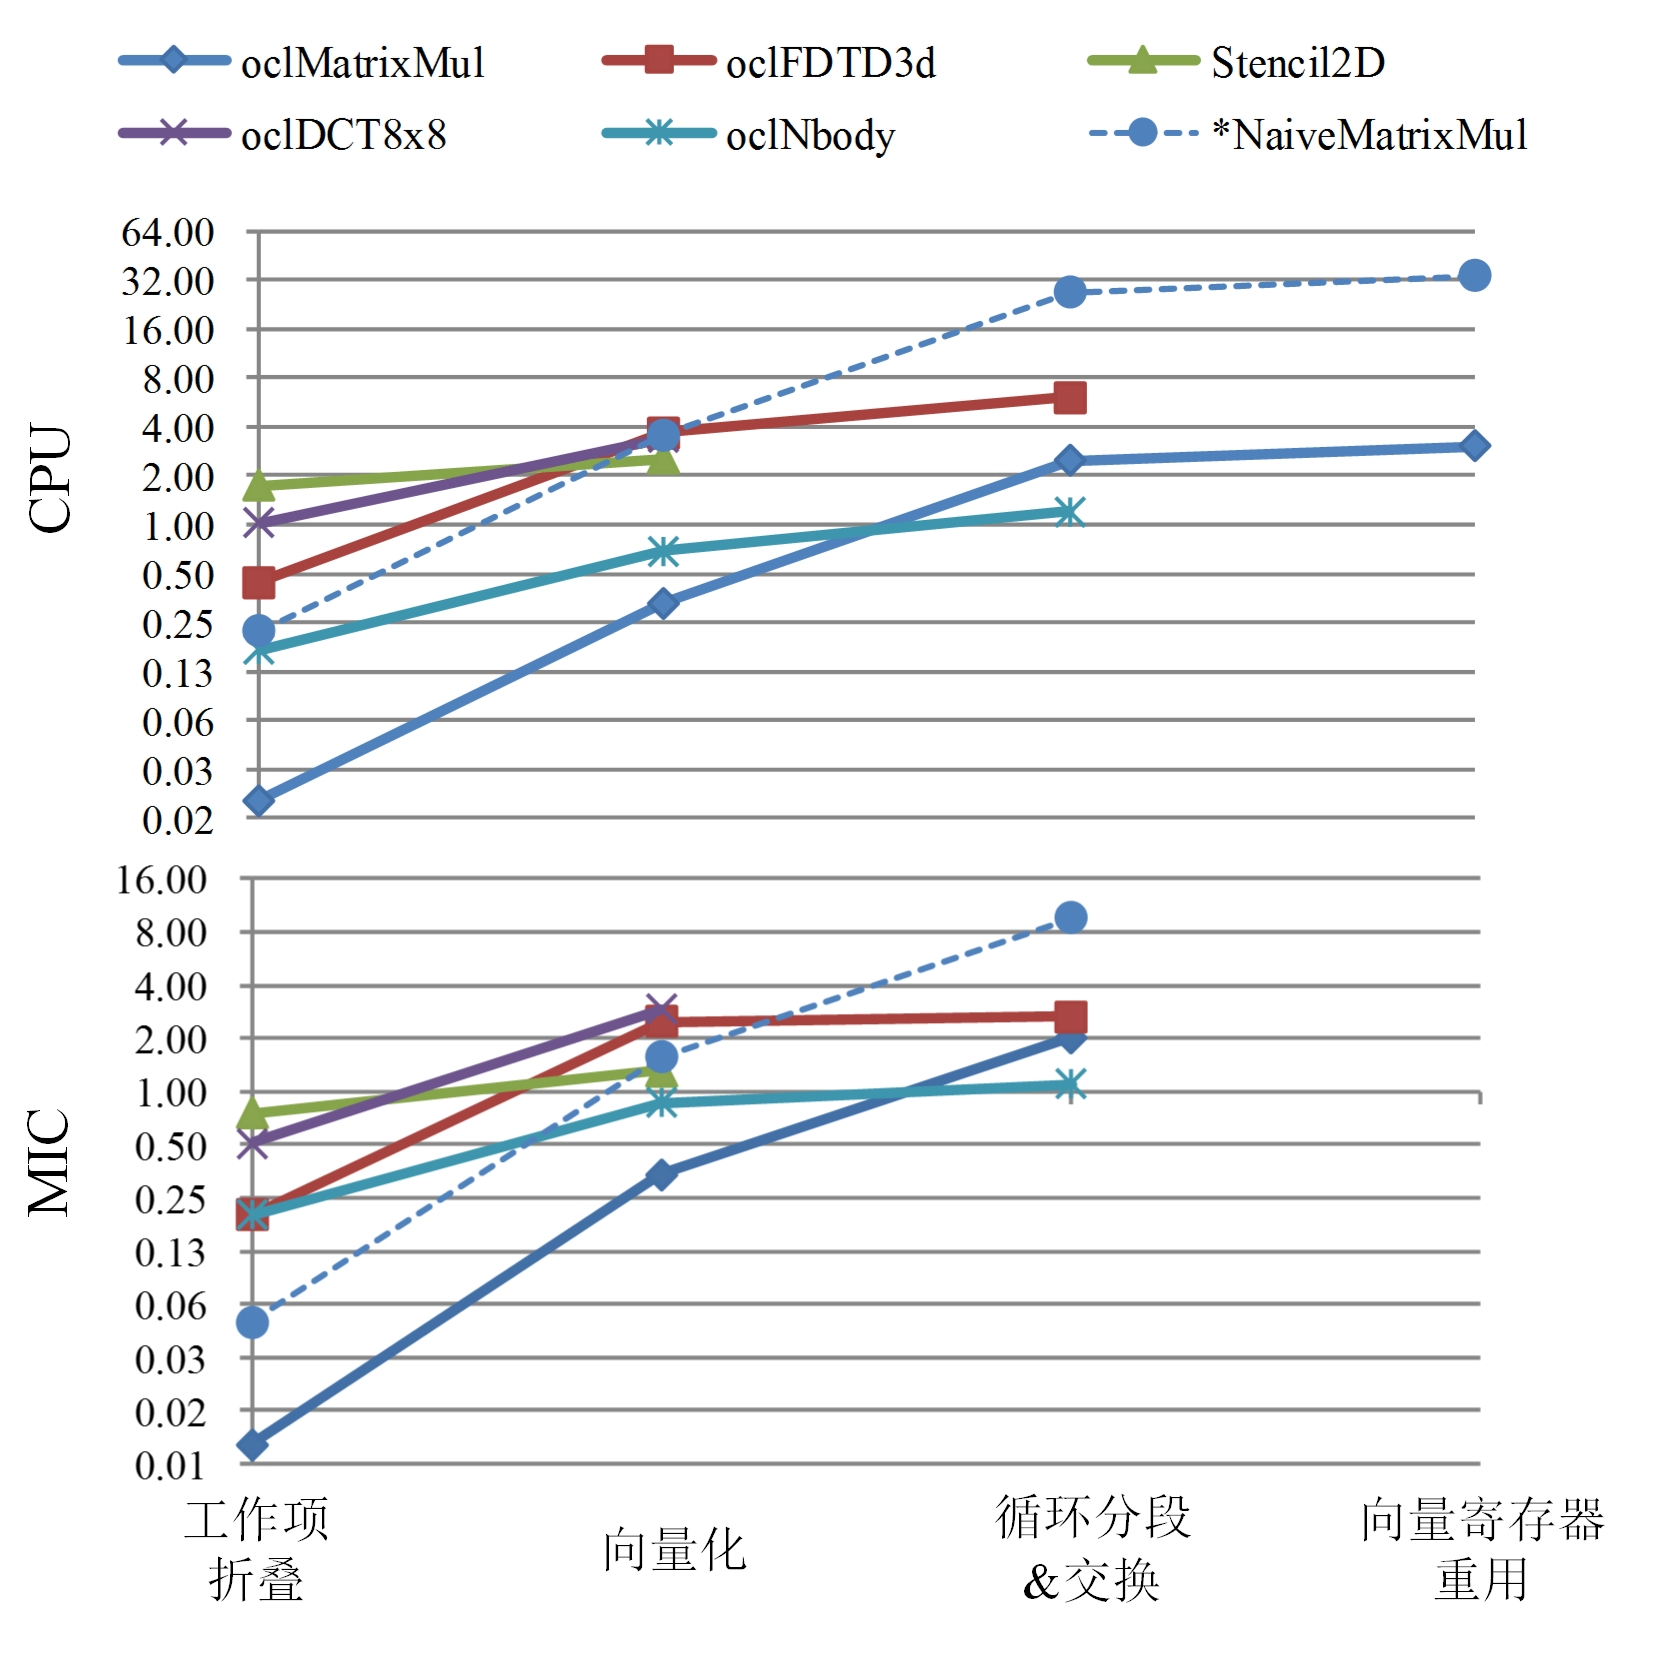
\includegraphics[width=11cm]{table3.jpg}
 	\caption{后继优化中各步骤带来的性能提升}
 	\label{asf}
 \end{figure}

根据图\ref{asf},向量化为oclMatrixMul和oclFDTD3d带来了巨大的性能提升,一些提升甚至超过了CPU的SIMD宽度。
原因在于向量化之前需要进行循环分布和交换,它们也会改变数据局部性,因此两种性能提升叠加在了一起。
但是,向量化对于oclNbody来说效果不明显,这是因为oclNbody中个体的速度和位置被紧邻地存储在一起,
即按``结构的数组''(Array of Structure)方式进行存储。
这将严重阻碍向量化的顺利进行。
NaiveMatrixMul的性能提升曲线和oclMatrixMul几乎一样,这是由于两者在工作项折叠后有着一样的控制流。
NaiveMatrixMul需要进行循环分段,而在循环分段后,两者的代码将变得相同。

\section{小结}
\label{kernelconclusionsec}
上一章中,通过在异构平台上基于OpenCL实现高性能TLD算法,OpenCL的性能移植性问题被暴露出来。
为此,本章进行了深入的探讨和解决。
本章提出了一套新的代码转换方法,该方法能够有效地提升GPU特定Kernel程序在多核/众核CPU上的性能移植性。
本章的方法解决了现有方法所忽略的两个问题:
一是在CPU上使用局部存储数组可能对性能带来的负面影响,即额外的数据拷贝和同步开销;
二是忽视或者盲目继承GPU特定Kernel中的数据局部性特征,都可能带来的性能损失。
借助于本章新提出的数组访问描述式,在工作项折叠过程中,所有的冗余局部存储数组和对应的同步都将被消除。
后继优化过程中,本章不仅从原GPU特定Kernel中提取并行性和局部性特征,还会考虑目标CPU的体系结构细节,
以进一步提升Kernel程序在CPU上的性能。
实验显示,无论对于经典的多核CPU,还是新兴的众核协处理器MIC,包含本章方法的新OpenCL运行时都能取得超越Intel官方
运行时的性能。
本章的方法仍然存在诸多不足,例如无法支持间接数组访问、静态调度算法不够高效、没有考虑工作组间的优化等。
未来将针对这些不足进行进一步的研究。
 
